\section{Resultate}

\todo{Kleiner Einleitungstext}



\subsection{Ergebnisse des Modelltrainings} \label{chap:ergebnisse-modelltraining}

Beim Modelltraining konnten wir keine Erfolge mit den VGG und den AlexNet Modellen erzielen, da diese Modelle nach dem Training alles als positiv klassifizieren. Der ViT führte beim COVIDx ebenfalls zu schlechten Ergebnissen, konnte aber den MRI Datensatz im Vergleich besser erlernen.

\begin{figure}[ht!]
    \centering
    \begin{subfigure}{0.5\linewidth}
        \centering
        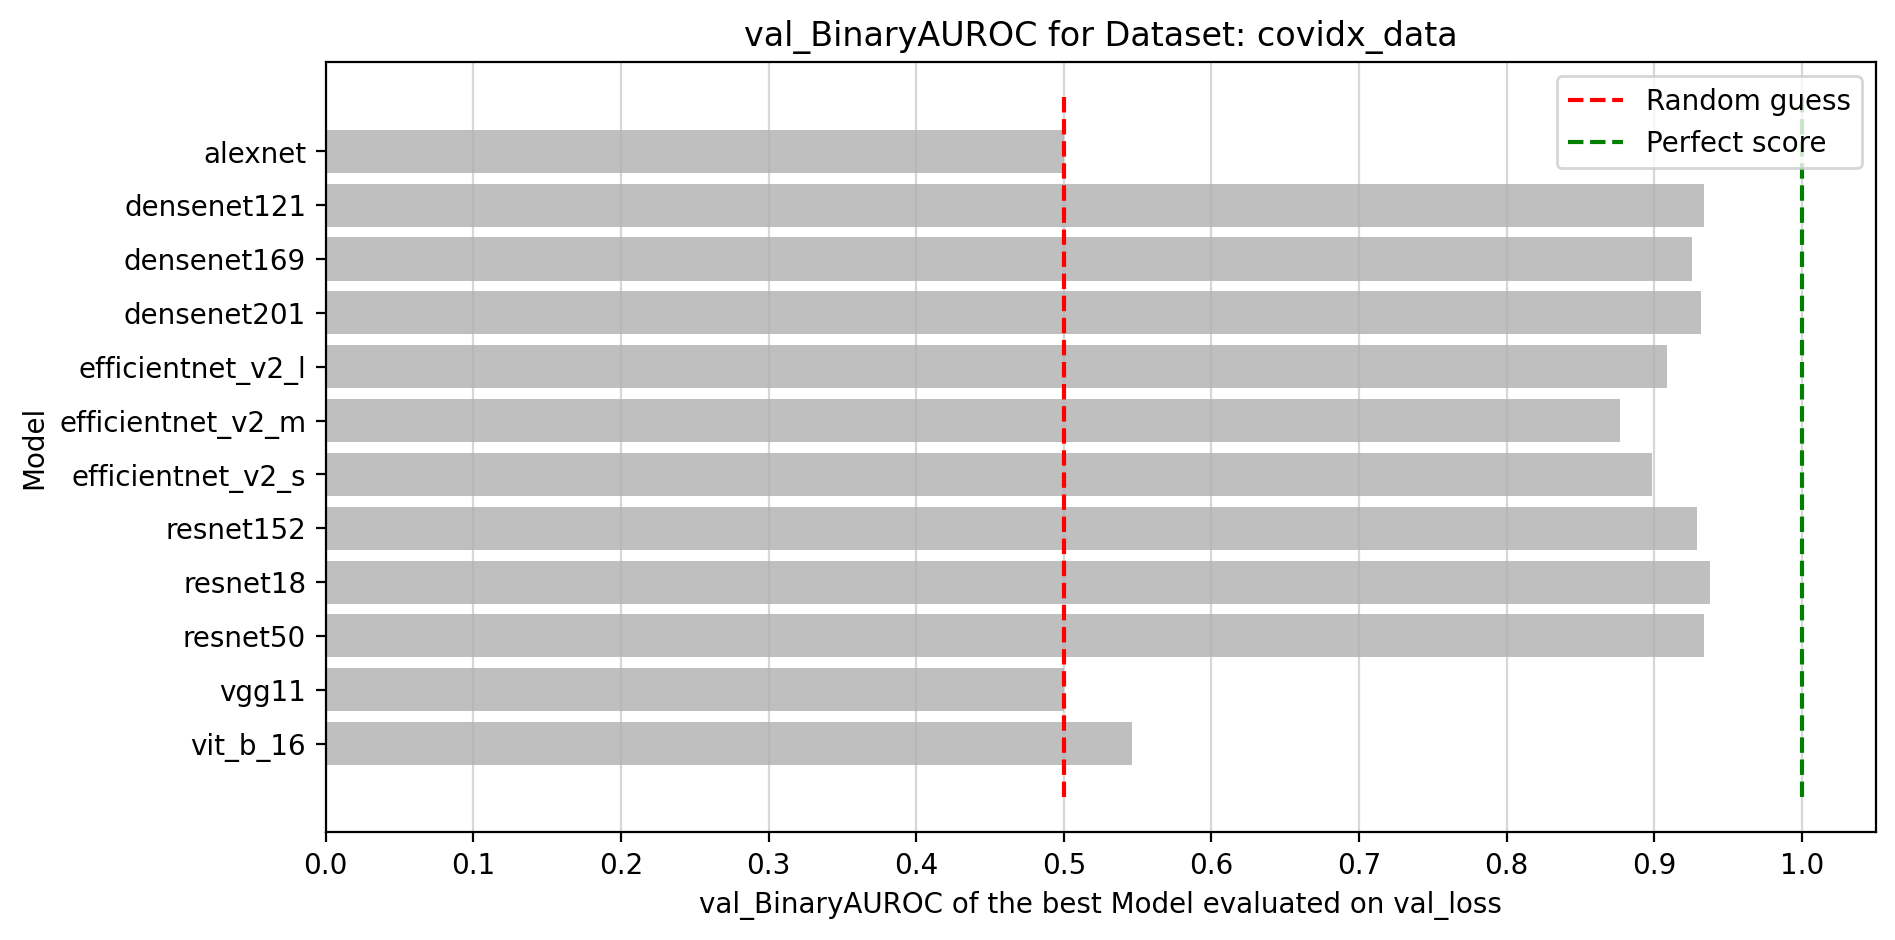
\includegraphics[height=0.5\linewidth]{01-images/05-resultate/val_binaryAUROC_COVIDX.png}
        \caption{...  für den COVIDx-Datensatz}
    \end{subfigure}\hfill%
    \begin{subfigure}{0.5\linewidth}
        \centering
        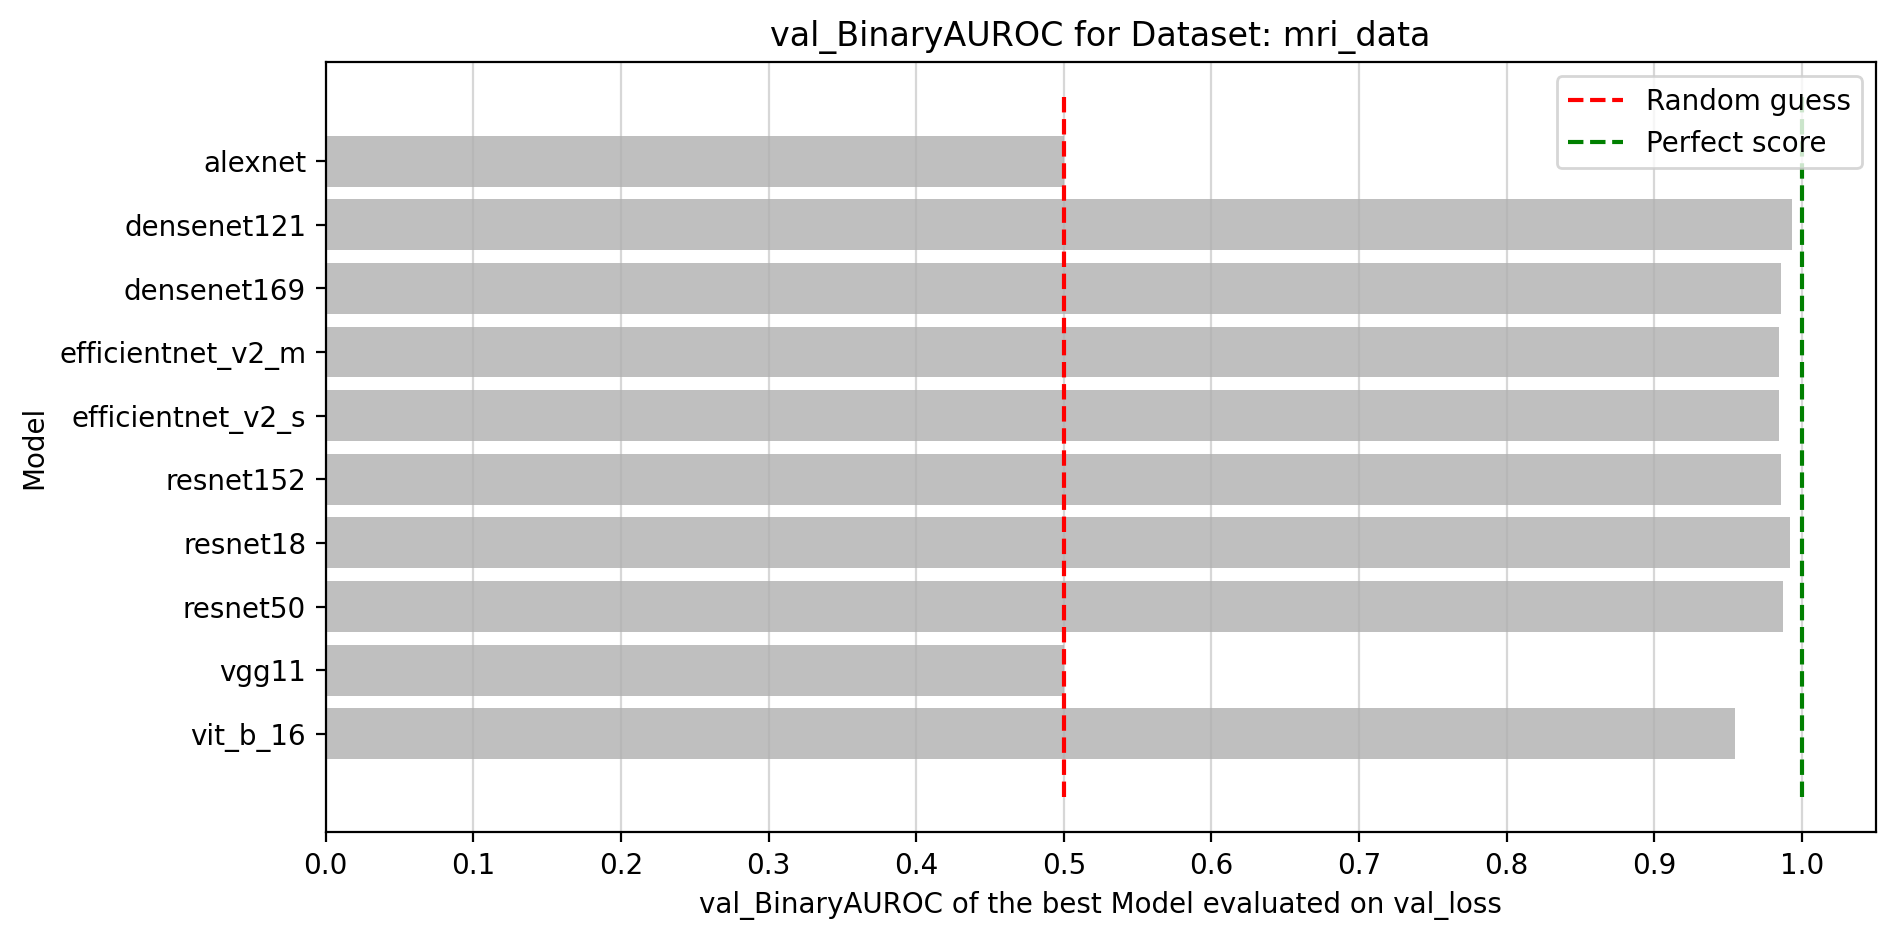
\includegraphics[height=0.5\linewidth]{01-images/05-resultate/val_binaryAUROC_MRI.png}
        \caption{... für den MRI-Datensatz}
    \end{subfigure}
    \caption{Die AUROC-Validierungsmetriken der besten Modelle im Trainingslauf (gemessen an der val\_loss-Metrik)}
\end{figure}

Wir sehen bei beiden Datensätzen eine Differenz zwischen den Validierungs- und den Testmetriken, wobei es scheint, als würden die Modelle auf den Validierungsdaten overfitten, obwohl beim Training nur die Lernrate optimiert wurde und das beste Modell mittels Checkpointing auf den Validierungsloss bestummen worde. Die Differenz könnte durch den möglichen Unterschied in den Distributionen der Partitionen, wie im Kapitel
\ref{chap:Datenverteilung-Testperformance-covidx}
und \ref{chap:Datenverteilung-Testperformance-mri} thematisiert, und erklärt werden.

\begin{figure}[ht!]
    \centering
    \begin{subfigure}{0.5\linewidth}
        \centering
        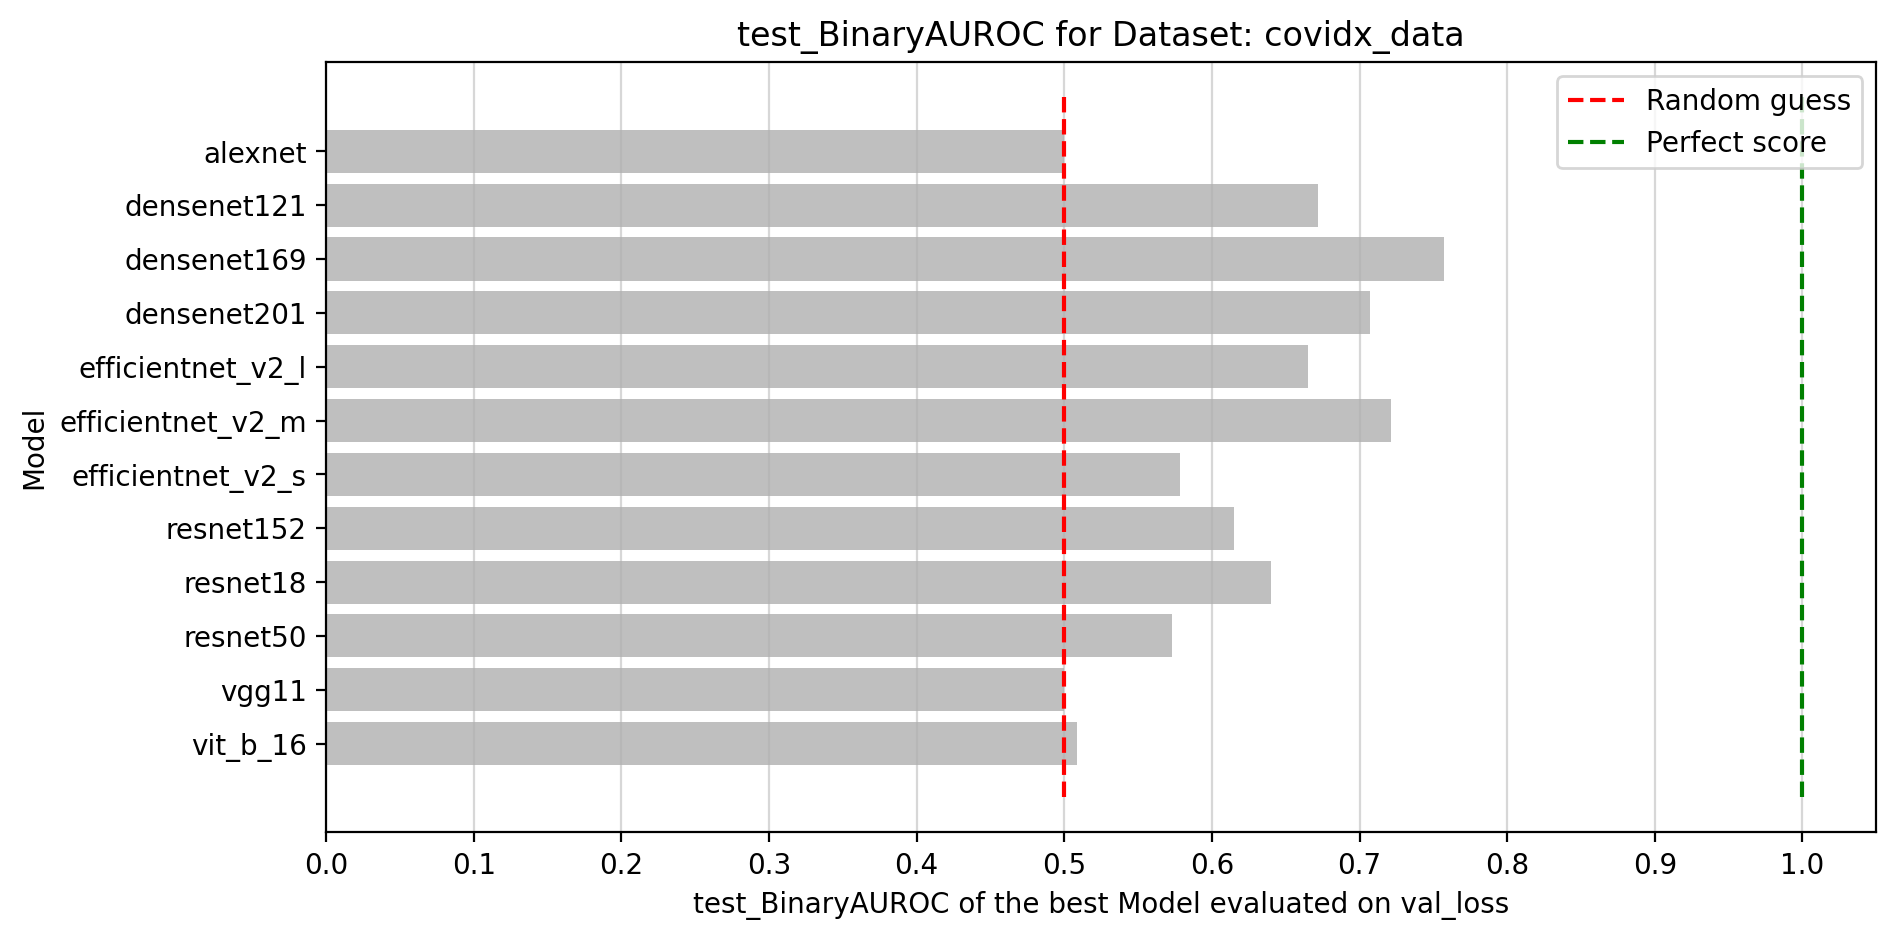
\includegraphics[height=0.5\linewidth]{01-images/05-resultate/test_binaryAUROC_COVIDX.png}
        \caption{...  für den COVIDx-Datensatz}
    \end{subfigure}\hfill%
    \begin{subfigure}{0.5\linewidth}
        \centering
        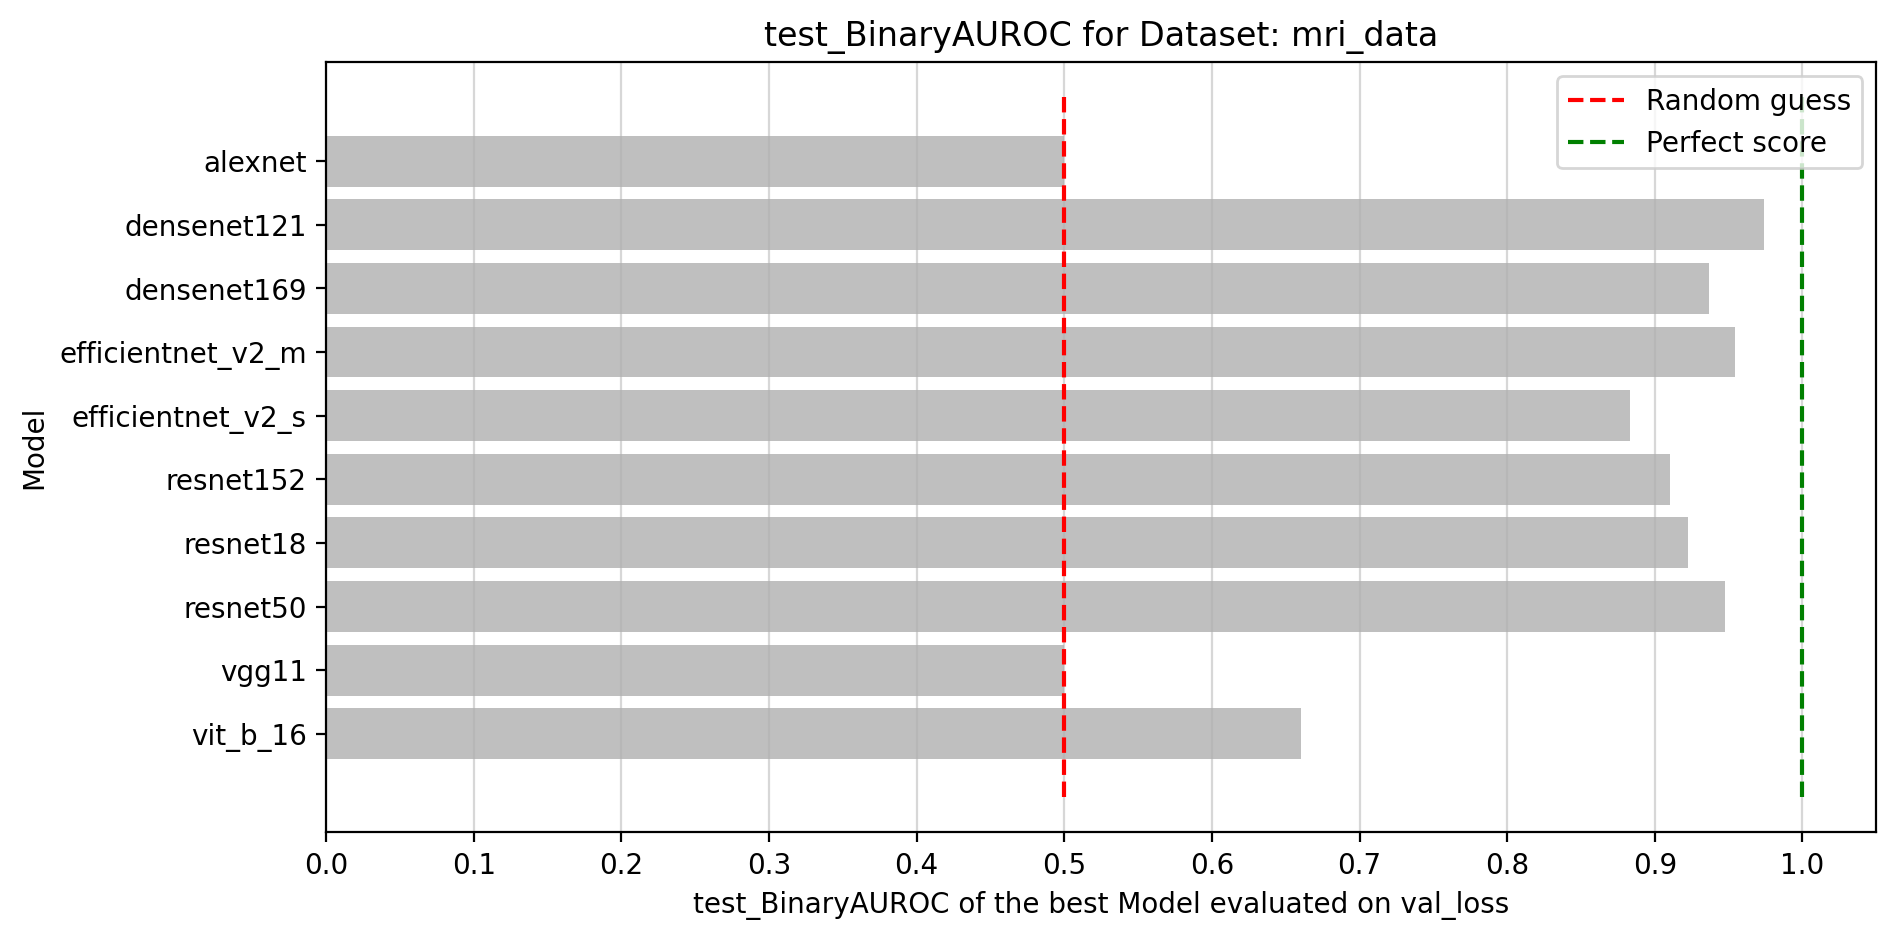
\includegraphics[height=0.5\linewidth]{01-images/05-resultate/test_binaryAUROC_MRI.png}
        \caption{... für den MRI-Datensatz}
    \end{subfigure}
    \caption{Die AUROC-Testmetriken der besten Modelle im Trainingslauf (gemessen an der test\_loss-Metrik)}
\end{figure}

Wegen den grossen Unterschieden zwischen dem Validierungs- und Testdatensatzes evaluieren wir die Anfälligkeit der Modelle auf beiden Datensätzen.

\newpage

\subsection{Universal Adversarial Perturbation}

\subsection{Anfälligkeit der ungeschützten Modellen}

\subsection{Anfälligkeit der geschützten Modellen}


\subsubsection{Adversarial Training}

\subsubsection{Input Ensembles}


\subsubsection{Data Augmentation}

\subsubsection{Weitere Verteidigungsmechanismen}


